\documentclass[10pt]{article}
\usepackage{hyperref}
\usepackage{listings}
\usepackage{biblatex}
\usepackage{tikz}
\usepackage{refstyle}
\usepackage{mathabx}
\usepackage{amssymb}
\usepackage{caption}
\usepackage{float}
\usepackage{graphics}
\usepackage{subfig}
\usepackage{enumitem}
\graphicspath{{/storage/FWC/digital-design/assembly/pf.tex}}
\begin{document}
\title{\textbf{GATE 2023 Computer Science and 
Information Technology (CS)}}
\date{\today}
\maketitle
\begin{enumerate}
    \item
    The output of a 2-input multiplexer is connected
back to one of its inputs as shown in the figure.

\begin{figure}[H]
\centering
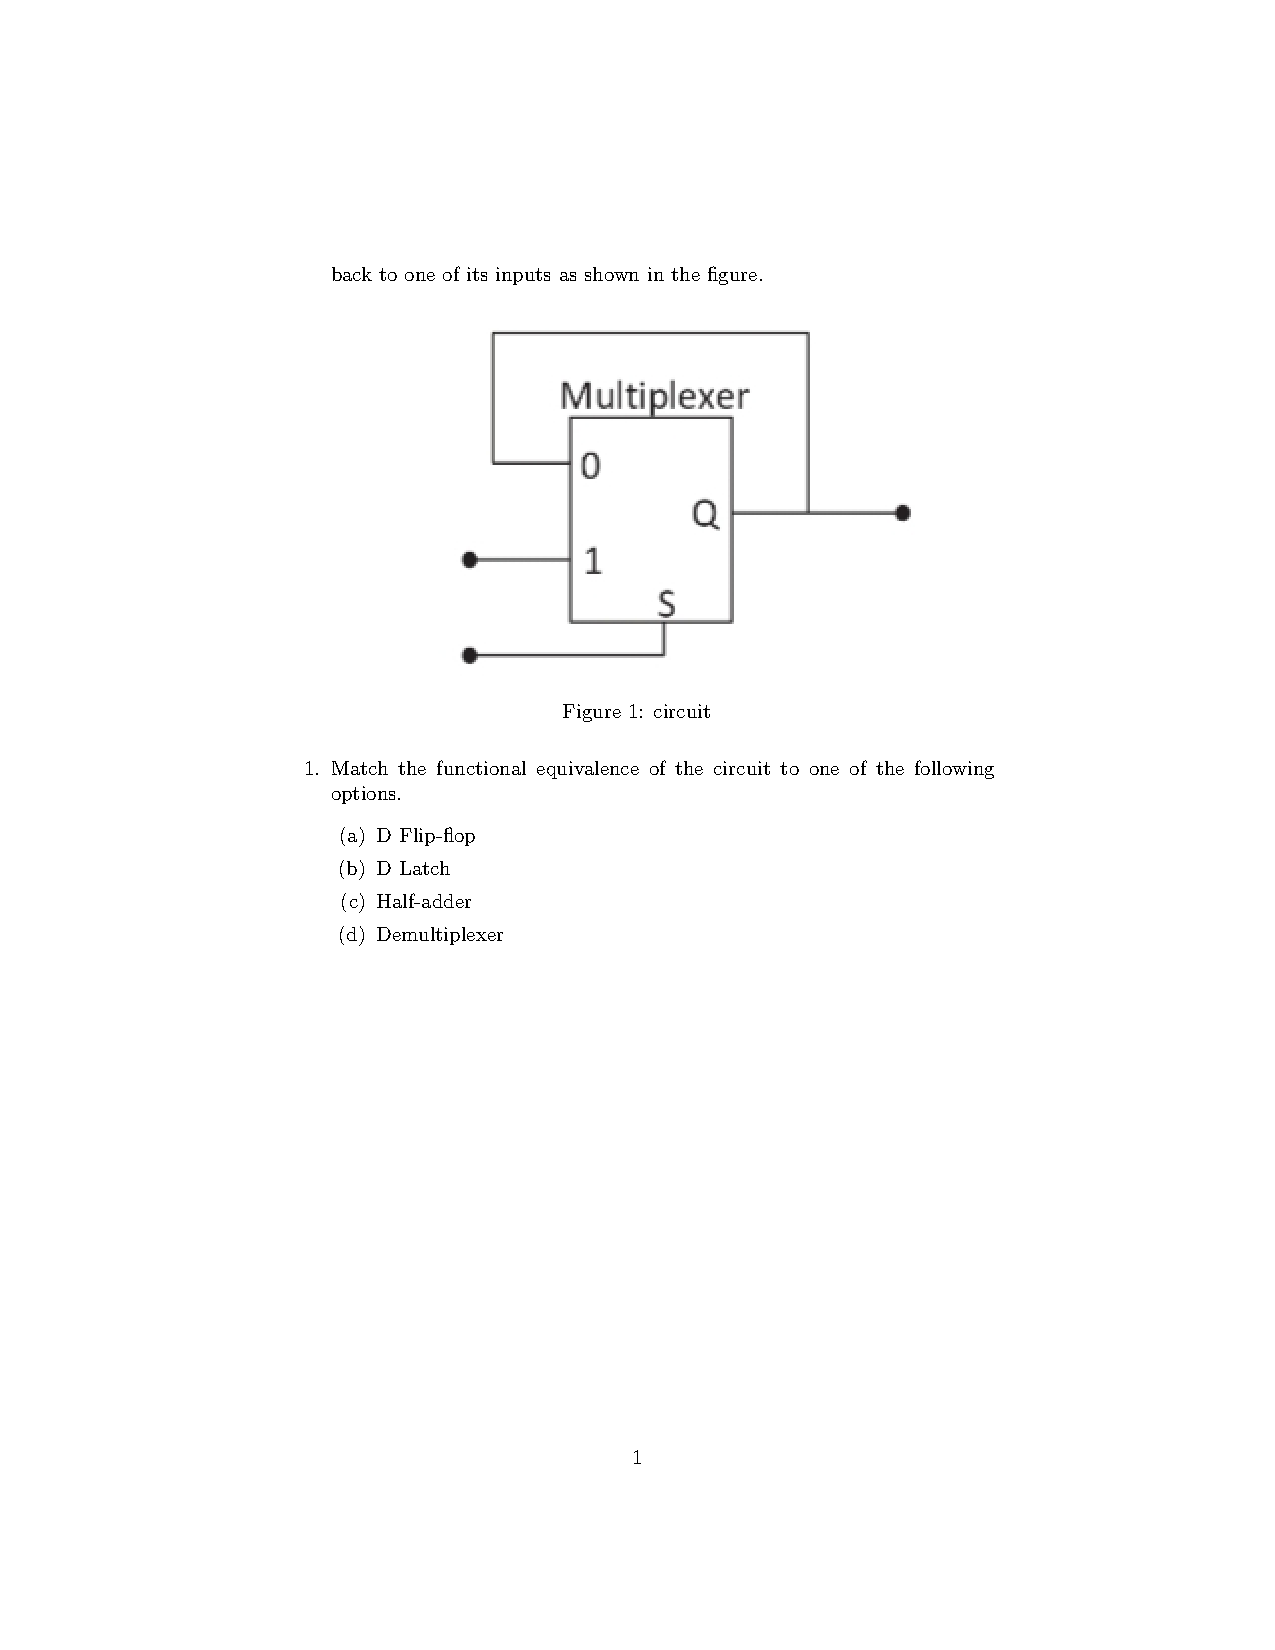
\includegraphics[width=\columnwidth]{/sdcard/FWC/digital-design/figs/pf.jpg}
\caption{circuit}
\label{fig:lcd}
\end{figure}
\item
 Match the functional equivalence of the circuit to
 one of the following options.

\begin{enumerate}
    \item D Flip-flop
    \item D Latch
    \item Half-adder
    \item Demultiplexer
\end{enumerate}
\end{enumerate}
\end{document}


